\algnewcommand{\LineComment}[1]{\State \(\triangleright\) #1}
% New definitions
\algnewcommand\algorithmicswitch{\textbf{switch}}
\algnewcommand\algorithmiccase{\textbf{case}}
\algnewcommand\algorithmicassert{\text{assert}}
\algnewcommand\Assert[1]{\State \algorithmicassert(#1)}%
% New "environments"
\algdef{SE}[SWITCH]{Switch}{EndSwitch}[1]{\algorithmicswitch\ #1\ \algorithmicdo}{\algorithmicend\ \algorithmicswitch}%
\algdef{SE}[CASE]{Case}{EndCase}[1]{\algorithmiccase\ #1}{\algorithmicend\ \algorithmiccase}%
\algtext*{EndSwitch}%
\algtext*{EndCase}%

% \graphicspath{{Figures/Multi/P2/}{./}} 

\chapter{Simultaneous Multiple Quantile Estimation}
\label{ch: multi_quant}

\graphicspath{{Figures/Multi/}{./}} 

When the estimation for only a single quantile value is not enough, the idea of multi-quantile estimation appears. 
In this chapter we introduce the problem of simultaneous multi-quantile estimation along with two related methods. This chapter is organised as follow:

Section~\ref{sec: multi_intro} introduces the multi-quantile estimation for streaming data, followed by a discussion on the basic ideas to attack this problem. The next two sections will show how it is solved by methods focusing on different aspects.

Section~\ref{sec: multi_shiftQ} shows the \textit{shiftQ} algorithm for simultaneous quantile estimation by implementing the idea similar to SGD.

Section~\ref{sec: multi_{p2}} shows the \textit{$P^2$} algorithm that solves the problem in a much different way.

Section~\ref{sec: multi_discussion} list the comparison between the two methods, the discussion about the problem and our conclusion.

\section{The problem and opportunity of multi-quantile estimation}
\label{sec: multi_intro}

In real life implementations, quantile estimation usually do not focus on a single quantile value. For example, a common request is to show the median (the $0.5$-quantile) of the distribution, and at the same time show the outlier boundaries at ends of the distribution, like the $0.1$- and $0.9$- quantiles. It is also highly possible that multiple quantile estimates are required for a data distribution analysis.

\begin{figure}[h]
    \centering
	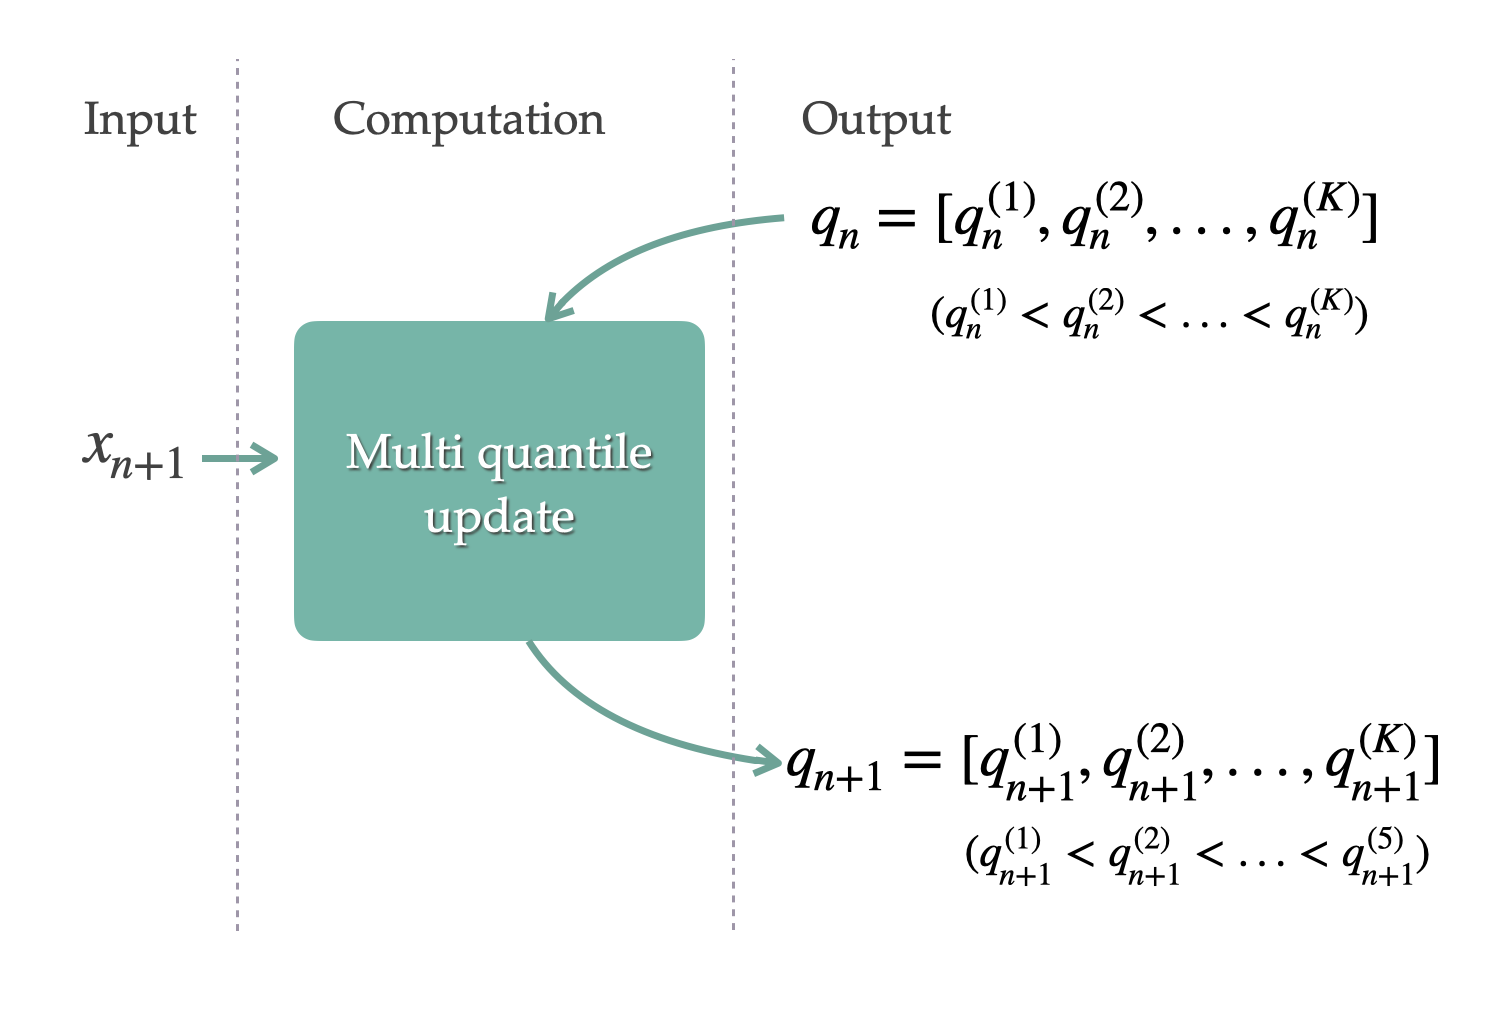
\includegraphics[width=0.7\columnwidth]{Multi_img.png}
	\caption{The update of multi-quantile estimation methods in general}
\end{figure}

A trivial solution for multi-quantile estimation is to run multiple single quantile estimation processes in parallel, such that each quantile is estimated by one process. The multi-process solution however, leads to two main problems:
\begin{enumerate}
    \item The parallel processing capacity of the implementation software/hardware.
    \item The missing information from the monotone property of quantiles.
\end{enumerate}

The following two multi-quantile estimation methods can simultaneously estimate multiple quantile numbers in one process with the utilization of the non-decreasing feature. Both algorithms, \textit{shiftQ}\cite{hammerJointTrackingMultiple2019b} and \textit{extended $p^2$}\cite{raatikainenSequentialProcedureSimultaneous1993} utilize the monotone property by ensuring a positive distance between one quantile and its previous quantile, such that 
$q_{i} - q_{i-1} > 0$. The algorithm explanation of the shiftQ algorithm is described in section \ref{sec: multi_shiftQ}, and the next section \ref{sec: multi_{p2}} for the extended $p^2$ algorithm.



% ----------------------------------- shiftQ ---------------------------------------

\section{The shiftQ method}
\label{sec: multi_shiftQ}

In general, shiftQ estimates a central quantile point, and update other quantiles based on the central one. The independent update of the central point is based on the deterministic update-based multiplicative incremental quantile estimator (DUMIQE) algorithm\cite{yazidiMultiplicativeUpdateMethods2019}, and the update of other quantiles implement the idea of shifted distributions. In this section, we first briefly introduce the DUMIQE algorithm, followed by the explanation of shifted distribution and then the approach of the shiftQ algorithm in section \ref{subsec: multi_shiftQ_description}.
\\\\
The DUMIQE algorithm updates the quantile estimate upon the arrival of each new observation. It is a development on the work of \citeauthor{tierneySpaceEfficientRecursiveProcedure1983}\cite{tierneySpaceEfficientRecursiveProcedure1983}, which applies a stochastic approximation on quantile estimation. The similarity between DUMIQE and SGD can be seen in the following algorithm pseudo-code:

\begin{algorithm}
    \caption{DUMIQE algorithm}\label{alg:DUMIQE}
    \begin{algorithmic}[1]
        \Require{Data Stream $X$, stepsize $\alpha$}, $\tau$, initial quantile estimate $q_0$ ($q_0 > 0$)
        \Ensure{$q$}
        % \Procedure{frugal}{$X,\tau$}            \Comment{X is the dataset}
        % \State {Initialize} $q$                 \Comment{Requires \textbf{positive initialization} $q$ > 0}
        \State{$q = q_0$}                         \Comment{\textbf{Positive} initialization }
            \For{$x_k$ in $X$}                  \Comment{Parameter update for each input data point}
                % \State \textbf{set} $\alpha_k$  \Comment{Set stepsize}
                \If{$x_k > q$}                  
                    \State{$q = q + \alpha \tau \cdot q$}
                \Else                           
                    \State{$q = q - \alpha (1-\tau)\cdot q$}
                \EndIf
            \EndFor
        \State \textbf{return} $q$              \Comment{$q$ is the DUMIQE estimation result}
    \end{algorithmic}
\end{algorithm}

The update of other quantiles are based on the the relationship with the central quantile. For example, if the central quantile is the median, the $0.25$-quantile is then estimated as the median of distribution below the estimate of median. To apply this idea, DUMIQE uses a shifted distribution $Y$ of the input $X$ such that $X = Y + \delta$, where $\delta$ is the shift constant. In the following method description, we use $Q_X(q)$ and  $Q_Y(q)$ to denote the estimate of $q$ on distribution $X$ and $Y$. In order to distinguish the quantile estimate on different distributions, the DUMIQE algorithm for the $\tau_k$-quantile on distribution $X$ at the observation of the $n$th sample $x_n$ is written as
\begin{align}
        &Q_{X, n+1}(q_k) \leftarrow Q_{X, n}(q_k) + \alpha \tau_k \cdot Q_{X, n}(q_k)  & \text{if } Q_{X, n}(q_k) < x_n \\
        &Q_{X, n+1}(q_k) \leftarrow Q_{X, n}(q_k) - \alpha (1-\tau_k) \cdot Q_{X, n}(q_k)  & \text{if } Q_{X, n}(q_k) \geq x_n \nonumber
\end{align}

\subsection{Method Description}
\label{subsec: multi_shiftQ_description}

\textbf{Motivation}: The difference between the two quantiles for the $x_{n}$ observation is:
$$
diff = |Q_{X,n}(q_{k+1}) - Q_{X,n}(q_k)|
$$
Note that $diff > 0$ for all $x_i, i \in \{1,...,N\}$, so different quantiles never cross each other. This property is guaranteed by the update function DUMIQE() and its restriction that the input quantile estimate must be positive.
\\\\
At the arrival of observation $x_n$, the central quantile estimate $q_c$ is first updated. Denote $K$ as the number of quantiles for estimation. Then the larger quantile estimates are updated on the smaller one in the sequence $\{q_{c-1}, ..., q_1\}$, and similarly the bigger quantile estimates are updated in the order of {$q_{c+1}, ..., q_{K}$}. The steps are:
\begin{enumerate}
    \item \textbf{Update the central quantile:} Calculate $q_c = Q_{X,n+1}(q_c)$ by DUMIQE
    \item  \textbf{Update one quantile}: The difference is calculated based on the idea of "shift distribution". Let $X$ denotes the original distribution of data stream, and let distribution $Y$ denotes a shifted version of $X$ such that $Y = X + constant$. In this way, the quantile estimate $q_{k+1}$ can be updated by implementation of shifting. The basic steps are:
        \begin{itemize}
            \item Calculate the shift constant $\delta = Q_{X,n}(q_k)$
            \item Get shift observation $y_{n,k+1} =  Q_{X,n}(q_k) - x_n$
            \item Calculate the shifted quantile estimate $Q_{Y, n+1}(q_{k+1})$ by DUMIQE
            \item Shift back to $X$: $Q_{X,n+1}(q_{k+1}) =  \delta  - Q_{Y, n+1}(q_{k+1})$
        \end{itemize}
    \item \textbf{Update the smaller quantiles:} Starting from central quantile $q_c$, the estimates for $q_{c-1}, ..., q_{1}$ are calculated one based on another. So each time step 2 is repeated from $q_c$ to $q_{2}$
    \item  \textbf{Update the bigger quantiles:} Similar to step 3, for smaller quantiles, estimates for $q_{c+1}, ..., q_{K}$ are calculated similarly one based on another.
\end{enumerate}

\subsection{The shiftQ Algorithm}
\begin{algorithm}
    \caption{The shiftQ Algorithm}\label{alg:multi_shiftQ}
        \begin{algorithmic}[1]
            \Require
            \State{Dataset $X$ (with positive data points only)}
            \State{Demanding quantile values $[\tau_1, \tau_2, ..., \tau_K]$}
            \State{Centeral position $c$, Number of quantiles $K$}
            \State{Stepsize $\alpha_X$, Stepsize $\alpha_Y$}
            \State{Quantile Estimate Initialization on $X$: {$0 < Q_{X,0}(q_1) < ... < Q_{X,0}(q_K)$}}
            \State{Quantile Estimate Initialization on $Y$: {$0 < Q_{Y,0}(q_1) < ... < Q_{Y,0}(q_K)$}}
            \Ensure{Demaning quantile estimates $[\tau_1\text{-}q, \tau_2\text{-}q, ..., \tau_K\text{-}q]$}

            \State
            \For{$x_n \in X$}
                \LineComment{Update central quantile}
                \State{$q_c \leftarrow DUMIQE(q_c, x_n, \tau_c, \alpha_X)$}
                \State{}

                \For{$k \in \{c-1, ..., 1\}$}
                \LineComment{Update smaller quantiles}
                    \State{$\delta \leftarrow Q_{X,n+1}(q_{k+1})$}
                    \State{$y_{n,k+1} \leftarrow Q_{X,n}(q_{k+1}) - x_n$}
                    \State{$Q_{Y, n+1}(q_{k}) \leftarrow DUMIQE(Q_{Y, n}(q_{k}), y_{n,k+1}, q_k, \alpha_Y)$}
                    \State{$Q_{X,n+1}(q_{k}) \leftarrow \delta - Q_{Y, n+1}(q_{k+1})$}
                \EndFor
                \State{}

                \For{$k \in \{c+1, ..., K\}$}
                \LineComment{Update bigger quantiles}
                    \State{$\delta \leftarrow Q_{X,n+1}(q_{k-1})$}
                    \State{$y_{n,k+1} \leftarrow  x_n - Q_{X,n}(q_{k-1})$}
                    \State{$Q_{Y, n+1}(q_{k}) \leftarrow DUMIQE(Q_{Y, n}(q_{k}), y_{n,k-1}, q_k, \alpha_Y)$}
                    \State{$Q_{X,n+1}(q_{k}) \leftarrow \delta + Q_{Y, n+1}(q_{k-1})$}
                \EndFor
            \EndFor

            \State
            \LineComment{Return final estimaton}
            \State{$[\tau_1\text{-}q, \tau_2\text{-}q, ..., \tau_K\text{-}q] \leftarrow [Q_{X,N}(q_1), ..., Q_{X,N}(q_K) ]$}
        \end{algorithmic}
\end{algorithm}
\subsection{Experiment Results}

There are two experiments run on shiftQ algorithm. The first one is aim to check the effect on quantile crossing reduction, and the second one tests the performance of quantile estimation.

In the first experiment, the experiment dataset is 5000 samples generated from a uniform distribution in range $(0,100)$. All data points are required to be positive as the pre-request of shiftQ algorithm. This experiment compares two algorithm, shiftQ and SGD, for the validation of crossing reduction of the shiftQ algorithm.

\begin{figure}[h]
	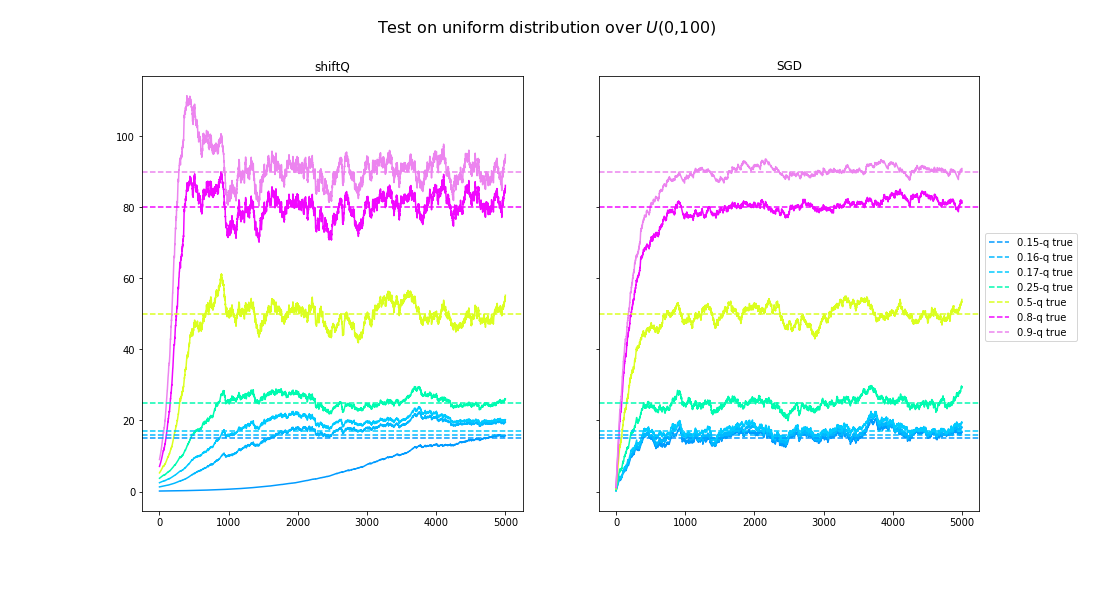
\includegraphics[width=1\columnwidth]{shiftQ/shiftQ_vs_SGD.png}
	\caption{The estimation comparison between shiftQ and SGD over a uniform distribution}
\end{figure}

In this experiment, $0$ crossing occurs in the shiftQ implementation, while 33 crossings happened over 5000 SGD estimation epochs. Over 100 experiments on the same data distribution over SGD, the average crossing number is 72.48, and the standard deviation is 66.23. The crossing in SGD has two interesting properties:
    \begin{enumerate}
        \item The crossings are likely to occur when two quantile values are close to each other. For example, in this example, only two pairs of quantiles ($0.15$, $0.16$) and ($0.16$, $0.17$) are detected to have crossings. The difference between two quantile values in the two crossing pairs are also 1, while the other adjacent quantile pairs are at least 8 away from each other. Given the setting of stepsize $\alpha = 0.45$ for SGD, the short distance between two adjacent quantile values are likely to be the main cause of crossings.
        \item The crossings happen are likely to happen in a slot of concentrated continuous epochs. For example, among the 33 crossings, 11 of them are between $0.16$-q and $0.17$-q from epoch 2400 to 2410. The other 22 crossings are between $0.15$-q and $0.16$-q continuously from epoch 3489 to 3510.It is implied that once a crossing takes place, its impact is likely to continue for the following epochs until the crossing is fixed.
    \end{enumerate}

The second experiment aims to show the effectiveness of shiftQ algorithm. Here are the plots of shiftQ algorithm on the absolute value of 1000 samples from Gaussian 1 distribution.

\begin{figure}[h]
	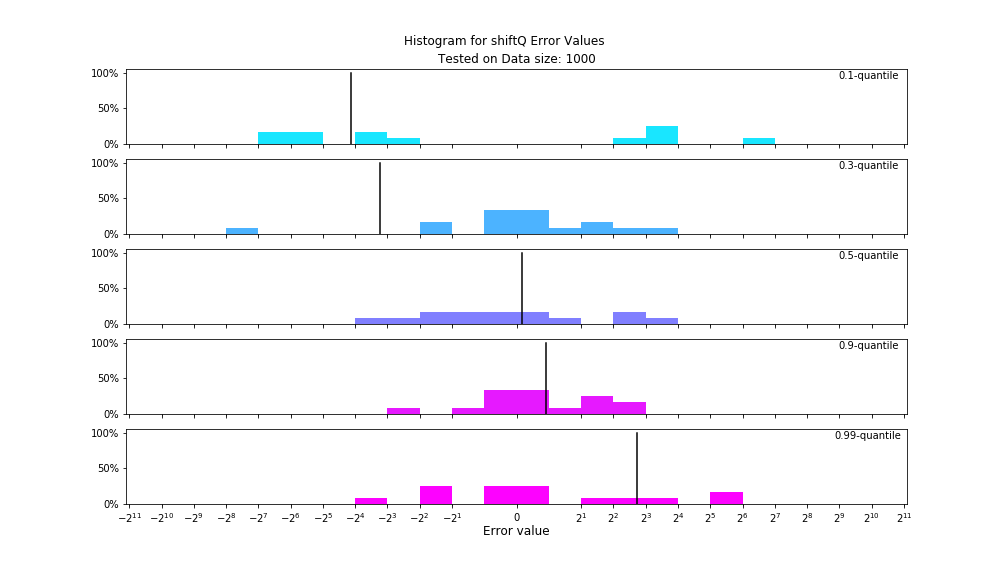
\includegraphics[width=1\columnwidth]{shiftQ/1000_err.png}
	\caption{The shiftQ algorithm for Positive Gaussian 1 distribution (the error graph)}
    \label{fig: shiftQ_err}
\end{figure}

\begin{figure}[h]
	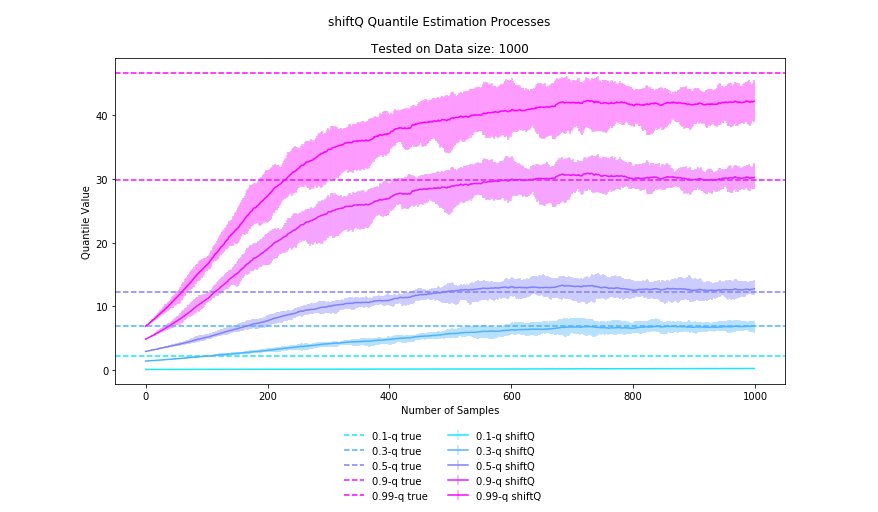
\includegraphics[width=1\columnwidth]{shiftQ/1000_proc.png}
	\caption{The shiftQ algorithm for Positive Gaussian 1 distribution (the process graph)}
    \label{fig: shiftQ_proc}
\end{figure}

\begin{figure}[h]
	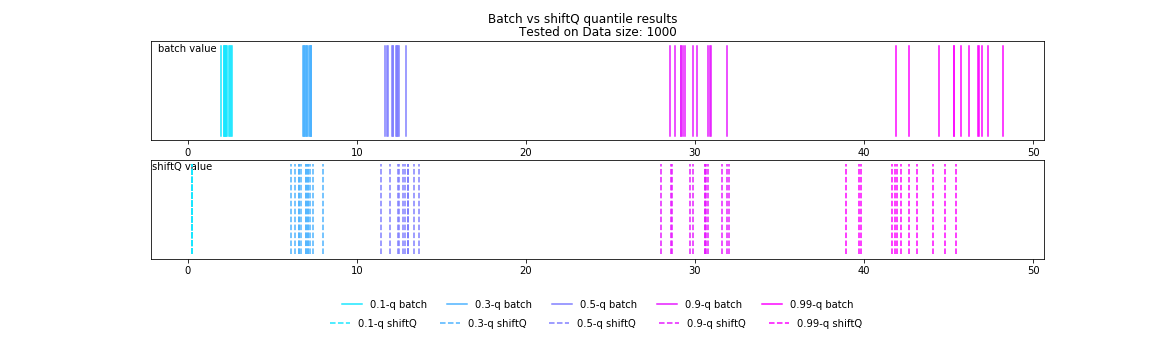
\includegraphics[width=1\columnwidth]{shiftQ/1000_res.png}
	\caption{The shiftQ algorithm for Positive Gaussian 1 distribution (the result graph)}
    \label{fig: shiftQ_res}
\end{figure}

It is shown in the Fig \ref{fig:shiftQ_err} that the shiftQ algorithm has a largely various performance on different quantiles. For example, the 0.5 and 0.9 quantiles has a much smaller and stable error distribution around 0, while the 0.1 quantile has a wide range of error values from less than -100 to more than 50. From the process plot Fig \ref{fig: shiftQ_proc} it is clear that the big error is not cause by the initialization value of 0.1-q. Instead, the estimation of 0.1-q has barely changed during the 1000 epochs. The converging trend of 0.99-q is also too slow to reach the true 0.99-q quantile at a higher value position. The distance between the batch quanitles and shiftQ estimated quantiles in Fig \ref{fig: shiftQ_res} has shown that the quantile estimates at both ends are far away from the computation.
% ----------------------------------- Extended P2 ---------------------------------------

\section{The Extended $P^2$ Algorithm}
\label{sec: multi_{p2}}

The \textit{Extended $P^2$} algorithm\cite{raatikainenSequentialProcedureSimultaneous1993} uses exactly the same idea of the $P^2$ algorithm\cite{jainP2AlgorithmDynamic1985}. So for a better understanding, we introduce the $P^2$ algorithm first in \ref{subsubsec: description_{p2}}, then the generation method for the extended $P^2$ algorithm.
In section \ref{subsec: algo_extended_{p2}}, the detailed algorithm for extended $P^2$ is provided, followed by its experiment results in section \ref{subsec: exp_extended_{p2}}.

\subsection{Method Description}

\subsubsection{The $P^2$ Method}
\label{subsubsec: description_{p2}}

The intuition of the $P^2$ method is the assumption that any three adjacent quantiles form a parabolic formula.
Specifically, the method interprets quantile estimation as a relationship based on quantile values and their ordering positions, and applies either linear or parabolic adjustments based on the information from their neighbours.

Suppose the straightforward quantile computation for [$\tau_1, ..., \tau_M$] that sorts all observations from the dataset $X = \{x_i\}^N_1$. Let $x_i$ denote the $i$th smallest value of $X$, then we have $x_1 < x_2 < ... < x_N$. 
To find the $\tau_i$-quantile of $X$, we need to find the data observation at \textit{marker position} $m_i = \tau_i \cdot N$. Given the marker position, we then retrieve the value of the marker, the corresponding \textit{quantile value} $q_i = x_{m_i}$. 
For 3 adjacent quantiles at $\tau_{i-1}, \tau_i, \tau_{i+1}$, their quantile values can be independently computed in the same way, as shown in Figure \ref{fig: {multi_relationship_p2}}.

\begin{figure}[h]
	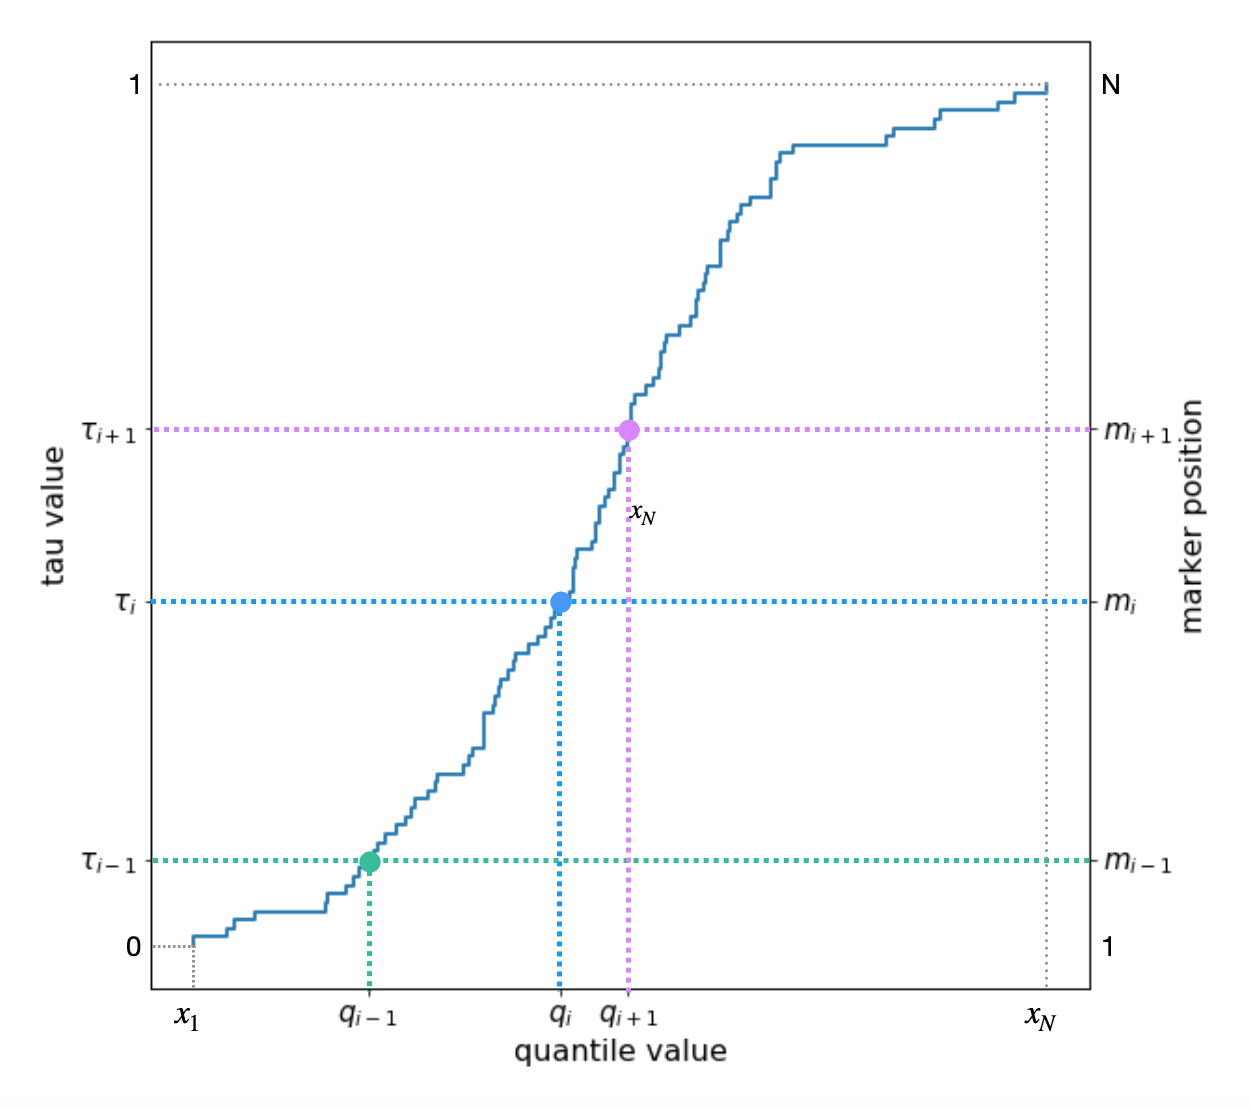
\includegraphics[width=0.8\columnwidth]{P2/relationships.png}
    \caption{Relationship between $\tau$ value, marker position and quantile values correspondingly for 3 adjacent quantiles}
    \label{fig: {multi_relationship_p2}}
\end{figure}

For quantile estimation, however, storing and sorting the entire dataset is infeasible. The $P^2$ method records only information only about demanding quantile values, and update them on the arrival of new observations. The update method, based on different conditions, is either a \textit{Piecewise-Parabolic} ($P^2$) formula, or a linear formula.

The information recorded for each quantile contains 3 parts: the marker position, the desired marker position, and the quantile value. For quantile $\tau_i$ with current observation number $M$, the desired marker position is $m_i \prime = 1 + (N-1)\tau$. This algorithm aims at keeping the marker position $m_i$ close to its desired position $m_i \prime$ while new observation coming in. The quantile value estimation $q_i$ is then updated accordingly after the current marker position is fixed. Figure \ref{fig: {multi_parabolic_p2}} demonstrates the update.

\begin{figure}[h]
    \centering
	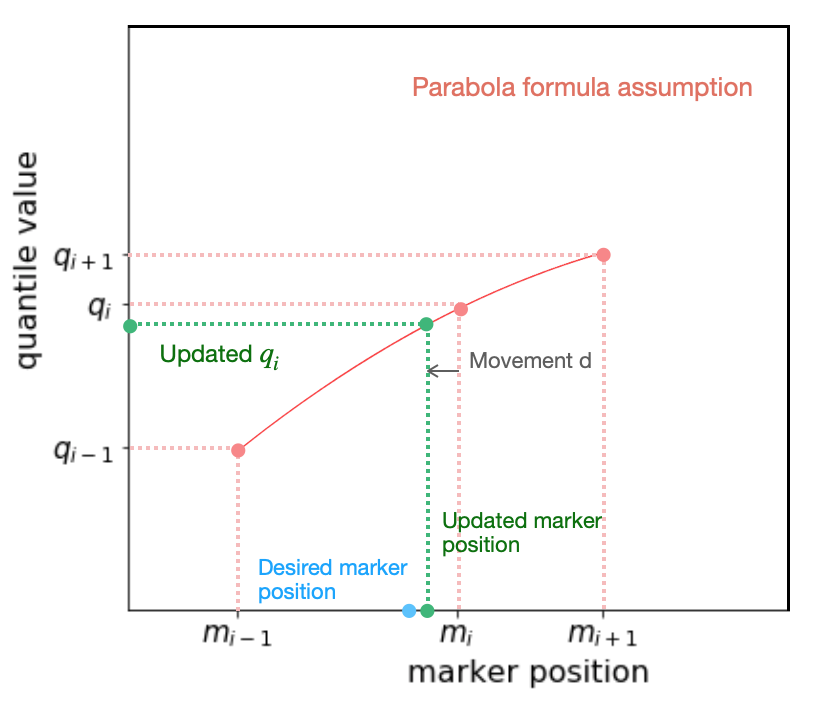
\includegraphics[width=0.7\columnwidth]{P2/parabola.png}
    \caption{Quantile value update using the Piecewise-Parabolic($P^2$) formula}
    \label{fig: {multi_parabolic_p2}}
\end{figure}

The quantile value update is based on the Piecewise-Parabolic assumption that any three adjacent makers form a parabolic curve of the form $q_i = aq_i^2 + bq_i + c$.

If a marker is moved $d$ positions to the right, the new quantile value is updated by:
\begin{align}
\begin{split}
    q_{i} \leftarrow q_{i}+ & \frac{d}{n_{i+1}-n_{i-1}}\\
    \cdot & { \bigg[ 
        \left(n_{i}-n_{i-1}+d\right) \frac{\left(q_{i+1}-q_{i}\right)}{\left(n_{i+1}-n_{i}\right)}
        +\left(n_{i+1}-n_{i}-d\right) \frac{\left(q_{i}-q_{i-1}\right)}{\left(n_{i}-n_{i-1}\right)}
        } \bigg] \\
    n_{i} \leftarrow n_{i}+&d \text{ where } d = \pm 1
\end{split}
\end{align}

When the parabolic assumption cannot be applied to the quantile value update, the altherative update is a piecewise-linear formula:
\begin{equation}
    \begin{array}{l}
    q_{i}=q_{i}+d \frac{\left(q_{i+d}-q_{i}\right)}{n_{i+d}-n_{i}} \\
    n_{i}=n_{i}+d
    \end{array}
\end{equation}

In short, the update method for $\tau_i$-quantile takes only 2 steps:\\
When a new observation comes,
\begin{enumerate}
    \item Update marker position $m_i$ to approach the desired marker position $m_i \prime$.
    \begin{enumerate}
        \item If the quantile value is bigger than the coming observation, move the marker position by one position to the right.
        \item Adjust the marker position again if it is more than one position away from the desired marker. The move $d$ is $1$ if the marker position moves right, and $-1$ for moving left.
    \end{enumerate}
    \item Update the quantile value
    \begin{enumerate}
        \item Try applying the parabolic update to the quantile value. Note it might change the non-decreasing order of quantiles, that is, $q_i \geq q_{i+1}$.
        \item If the ordering of quantile values is changed by the parabolic update, try the linear update instead.
    \end{enumerate}
\end{enumerate}


\subsubsection{The Extended $P^2$ Method}
In $P^2$, the update of a quantile relies on its position relative to the neighbour markers, indicating the accuracy of neighbour marker positions is important. 
It sets one marker for each quantile value, that is, a total of $M$ markers for [$\tau_1, ..., \tau_m$].
The extended $P^2$ algorithm improves the estimation accuracy by the introduction of "middle markers",  which nearly doubles the amount of markers in $P^2$. 
It means, in the initialization part, there will be $2M+3$ markers for
$$
\tau = 0, \frac{0+\tau_1}{2}, \tau_1, \frac{\tau_1 + \tau_2}{2}, \tau_2, ..., \tau_{M}, \frac{\tau_M+1}{2}, 1
$$
And the estimation update for all those markers follows the exact rule in the $P^2$ algorithm.

The only difference between extended $P^2$ and $P^2$ is the extension of markers at the initialization stage. At a doubly expensive computation cost, the quantile estimation reaches a higher accuracy from the extra information, as shown in the work of \citeauthor{raatikainenSequentialProcedureSimultaneous1993}\cite{raatikainenSequentialProcedureSimultaneous1993}. Besides the extra information brought by the extra markers, the extended $P^2$ algorithm also benefits from a better initialization by a larger sampling. The larger sampling in extended $P^2$ reduces the possibility of severely unevenly distributed initializations, which becomes important for  $P^2$, as it is sensitive to the initialization of quantiles.
% In $p^2$, only desired quantiles have their information recorded and used for 

\subsection{The Algorithm of Extended $P^2$}
\label{subsec: algo_extended_{p2}}

\begin{algorithm}
    \caption{The $P^2$ Algorithm}\label{alg:multi_p2}
        \begin{algorithmic}[1]
            \Require{Dataset $X$, $M$ Demanding quantile values $[\tau_1, \tau_2, ..., \tau_M]$}
            \Ensure{Demaning quantile estimates $[\tau_1\text{-}q, \tau_2\text{-}q, ..., \tau_M\text{-}q]$}
            \State
            \State{\textbf{A. Initialization}}
            \State {The first M observations (sorted): \{$x_1,x_2,...,x_M$\}}
            \For{$(i = 1, ..., M-1)$}
                \State {Marker height:    $q_i = x_i $}
                \State {Marker position:   $m_i = i$}
                \State {Desired Marker position:  $m_i\prime = (m-1)\tau_i + 1$}
            \EndFor

            \State
            \State{\textbf{B. For each new observation $x_j$, $j \geq M+1$, perform the following}}
            \Switch{$s$}            \Comment {Find the cell $k$ such that $q_k \leq x_j < q_{k+1}$}
                \Case{$x_j < q_1$}
                    \State{$q_1 = x_j, k = 1$}
                \EndCase
                \Case{$q_i \leq x_j < q_{i+1}$}
                    \State {$k = i$}
                \EndCase
                \Case{$q_M < x_j$}
                    \State {$q_M = x_j, k = M-1$}
                \EndCase
            \EndSwitch
            \State
            
            \State{$m_i = m_i + 1$; $i = k+1, ..., M$}       \Comment{Increment some marker positions}
            % \Comment{Different from that on the $P^2$ paper}
            \State{$m_i\prime = m_i\prime + \tau_i$}            \Comment{Update all the desired positions}

            \State
            \State{Adjust marker heights $2$ to $M-1$ if necessary:}
            \For{$i = 2, 3, ..., M-1$}
                \State {$d_i = m_i\prime - m_i$}
                \If {($ d_i \geq 1 \text{ and }  m_{i+1} - m_i > 1$) or 
                     ($ d_i \leq -1 \text{ and }  m_{i-1} - m_i < -1$) }
                    \State {$d_i = sign(d_i)$}
                    \State {$q_i\prime = \text{parabolic}(q_1)$}     \Comment{Try the $P^2$ update}
                    \If {$ q_{i-1} < q_i\prime < q_{i+1}$}
                        \State {$q_i = q_i\prime$}
                        \Else                           \Comment{Else use linear update}
                            \State{$q_i = \text{linear}(q_i)$}
                    \EndIf
                    \State {$m_i = m_i + d_i$}          \Comment{Update marker position}
                \EndIf
            \EndFor

            \State
            \State {\textbf{C. Return quantile estimates} }     
            \LineComment{The result is available after any number of observations}
            \State {$[\tau_1\text{-}q, \tau_2\text{-}q, ..., \tau_M\text{-}q] = [q_1, q_2, ..., q_M]$}
        \end{algorithmic}
\end{algorithm}

\begin{algorithm}
    \caption{Extended $P^2$ Algorithm}\label{alg:multi_ext_p2}
        \begin{algorithmic}[1]
            \Require{Dataset $X$, Demanding quantile values $[\tau_1, \tau_2, ..., \tau_M]$}
            \Ensure{Demaning quantile estimates $[\tau_1\text{-}q, \tau_2\text{-}q, ..., \tau_M\text{-}q]$}

            \State
            \State {\textbf{0.Extend number of markers from $M$ to $2M+3$}}
            \LineComment{Evenly fill the intervals between $0,1$ and each 2 quantile values}
            \State{$[\tau_1\prime, \tau_2\prime, ..., \tau_{2M+3} \prime] = [0, \frac{0+\tau_1}{2}, \tau_1, \frac{\tau_1 + \tau_2}{2}, \tau_2, ..., \tau_{M}, \frac{\tau_M+1}{2}, 1]$}

            \State
            \State{\textbf{1. Apply $P^2$ with the extended initialization}}
            \LineComment{And returns an estimate of extended list}
            \State{$[q_1\prime, ..., q_{2M+3}\prime] = P^2$ ($X$, $[\tau_1\prime, \tau_2\prime, ..., \tau_{2M+3} \prime]$)}
            \State
            \State {\textbf{2. Return quantile estimates} } 
            \State {Extract the quantile estimates for the original $M$ quantile values}
            \State {$[\tau_1\text{-}q, \tau_2\text{-}q, ..., \tau_M\text{-}q] = [q_3\prime, q_5\prime, ..., q_{2M+1}\prime]$}
        \end{algorithmic}
\end{algorithm}

% 0, 0.5, 1, 1.5, 2, ..., M,    (M+1)/2, 1
% 1, 2,   3, 4,   5, ..., 2M+1, 2M+2,   2M+3            

\subsection{Experiment Results}
\label{subsec: exp_extended_{p2}}
The $P^2$ algorithm is tested on the Gaussian 1 distribution on 1000 samples. And the results are shown in the following plots:
\begin{figure}[h]
	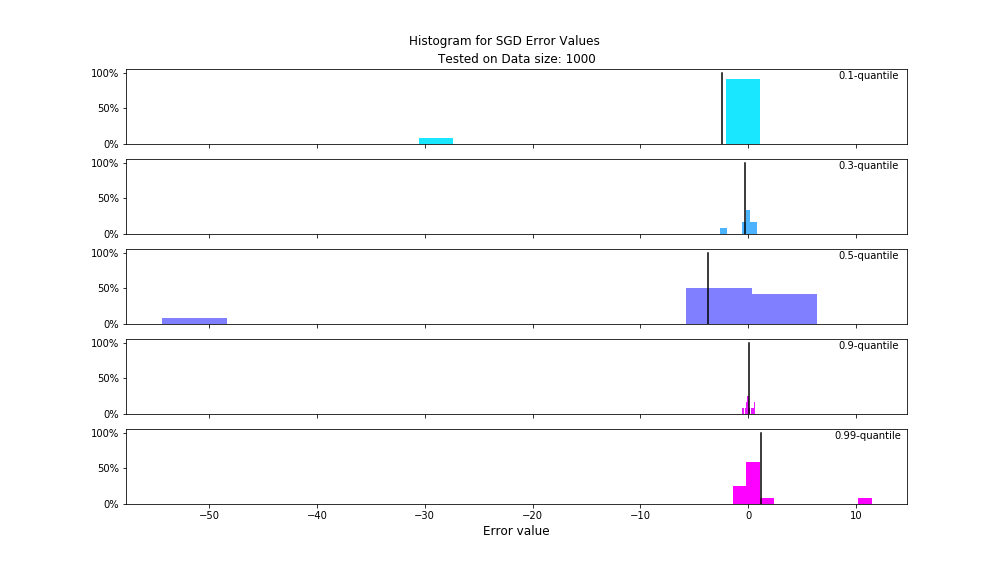
\includegraphics[width=1\columnwidth]{P2/1000_err.png}
	\caption{The P2 algorithm for Gaussian (mean = -20, std = 1)}
\end{figure}



\begin{figure}[h]
	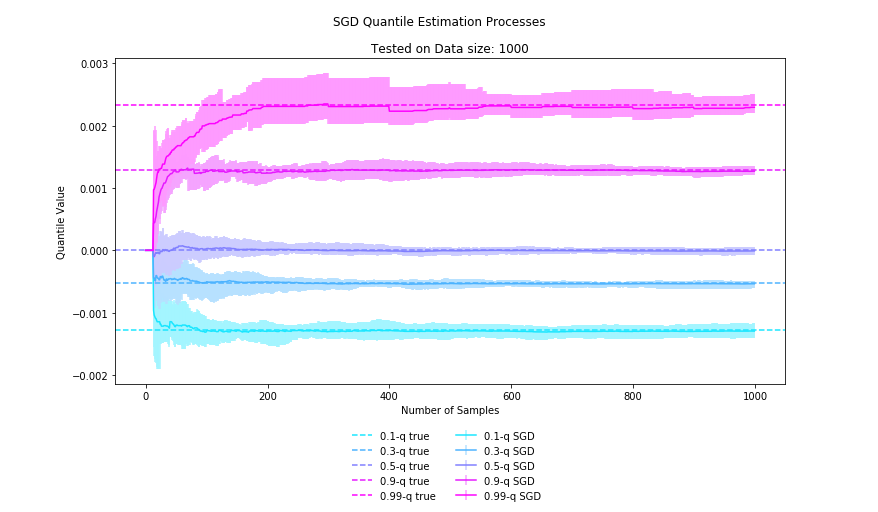
\includegraphics[width=1\columnwidth]{P2/1000_proc.png}
	\caption{The P2 algorithm for Gaussian (mean = -20, std = 20)}
\end{figure}

\begin{figure}[h]
	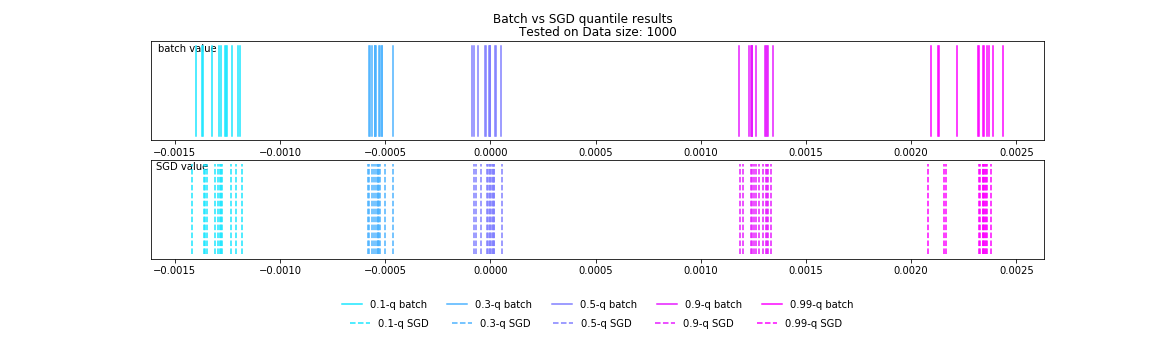
\includegraphics[width=1\columnwidth]{P2/1000_res.png}
	\caption{The P2 algorithm for Gaussian (mean = -20, std = $0.001$)}
\end{figure}

\section{Discussion and Conclusion}
\label{sec: multi_discussion}

From the experimental results we can see the two multi-quantile estimation methods can solve the crossing problem by introducing some mathematical relationship assumptions between adjacent quantiles. The following step will be doing nothing but to 